\section{Vector Spaces}

\begin{paracol}{2}

\begin{tikzpicture}
\node [rounded-box] (box){\begin{minipage}{0.45\textwidth}
    Let $V$ be a set on which two operations, addition and scalar multiplication, are defined. If the following axioms hold for all vectors $\mathbf{u}, \mathbf{v}, \mathbf{w} \in V$ and scalars $c, d$, then $V$ is called a vector space and its elements are called vectors. \\

    \begin{itemize}
        \item Closure under addition: $\mathbf{u} + \mathbf{v} \in V$
        \item Commutativity: $\mathbf{u} + \mathbf{v} = \mathbf{v} + \mathbf{u}$
        \item Associativity: $(\mathbf{u} + \mathbf{v}) + \mathbf{w} = \mathbf{u} + (\mathbf{v} + \mathbf{w})$
        \item There exists an element $\mathbf{0} \in V$, called the zero vector, such that $\mathbf{u} + \mathbf{0} = \mathbf{u}$.
        \item For each $\mathbf{u} \in V$, there exists an element $-\mathbf{u} \in V$ s.t. $\mathbf{u} + (- \mathbf{u}) = \mathbf{0}$.
        \item Closure under scalar multiplication: $c \mathbf{u} \in V$
        \item Distributivity: $c (\mathbf{u} + \mathbf{v}) = c \mathbf{u} + c \mathbf{v}$
        \item Distributivity: $(c + d) \mathbf{u} = c \mathbf{u} + d \mathbf{v}$
        \item $c(d \mathbf{u}) = (cd) \mathbf{u}$
        \item $1 \mathbf{u} = \mathbf{u}$
    \end{itemize}
\end{minipage}};
\node[rounded-box-title, left=10pt] at (box.north east) {Definition};
\end{tikzpicture}

\switchcolumn

\begin{tikzpicture}
\node [rounded-box] (box){\begin{minipage}{0.45\textwidth}
    Let $V$ be a vector space, $\mathbf{u}$ a vector in $V$, and $c$ a scalar. Then \\

    \begin{itemize}
        \item $0 \mathbf{u} = \mathbf{0}$
        \item $c \mathbf{0} = \mathbf{0}$
        \item $(-1) \mathbf{u} = - \mathbf{u}$
        \item If $c \mathbf{u} = \mathbf{0}$, then $c = 0$ or $\mathbf{u} = \mathbf{0}$.
    \end{itemize}
\end{minipage}};
\node[rounded-box-title, left=10pt] at (box.north east) {Theorem};
\end{tikzpicture}

A vector space consists of a set of vectors and all linear combinations of these vectors, and is equipped with operations of addition and scalar multiplication, satisfying certain properties like closure under addition and scalar multiplication, associativity, commutativity, and distributivity.

A linear subspace is a subset of a vector space operating that is itself a vector space. It retains all the properties of a vector space - within that subset, and it operates within the context of a larger vector space.

\end{paracol}

\subsection{Subspaces}

A subset of a vector space, $S \subseteq V$, can be described in the form $S = \{ \mathbf{v} \in V | \langle\ \text{some condition} \rangle \}$.

A subspace of a vector space, $W \subseteq V$, is a \textit{subset with vector space structure}, meaning it is closed under addition (for all $\mathbf{w}_1, \mathbf{w}_2 \in W, \mathbf{w}_1 + \mathbf{w}_2 \in W$) and scalar multiplication (for all $\mathbf{w} \in W, \lambda \in \mathbb{R}, \lambda \mathbf{w} \in W$). You can take arbitrary elements in the set, scale or add them together, and obtain an element of the same set.

\begin{paracol}{2}

\begin{tikzpicture}
\node [rounded-box] (box){\begin{minipage}{0.45\textwidth}
    A subset $W$ of a vector space $V$ is called a subspace of $V$ if $W$ is itself a vector space with the same scalars, closure under addition and scalar multiplication as $V$.
\end{minipage}};
\node[rounded-box-title, left=10pt] at (box.north east) {Definition};
\end{tikzpicture}

Checking whether a subset $W$ of a vector space $V$ is a subspace of $V$ involves testing only two of the ten vector space axioms.

\begin{tikzpicture}
\node [rounded-box] (box){\begin{minipage}{0.45\textwidth}
    Let $V$ be a vector space, and let $W$ be a non-empty subset of $V$. Then $W$ is a subspace of $V$ if and only if: \\

    \begin{enumerate}
        \item If $\mathbf{u}, \mathbf{v} \in W$, then $\mathbf{u} + \mathbf{v} \in W$.
        \item If $\mathbf{u} \in W, c \in \mathbb{R}$, then $c \mathbf{u} \in W$.
    \end{enumerate}
\end{minipage}};
\node[rounded-box-title, left=10pt] at (box.north east) {Theorem};
\end{tikzpicture}

\switchcolumn

\begin{tikzpicture}
\node [rounded-box] (box){\begin{minipage}{0.45\textwidth}
    If $S = \{ \mathbf{v}_1, \dots, \mathbf{v}_k \}$ is a set of vectors in a vector space $V$, then the set of linear combinations of $\mathbf{v}_1, \dots, \mathbf{v}_k$ is called the span of $\mathbf{v}_1, \dots, \mathbf{v}_k$, denoted by $\text{Span}(\mathbf{v}_1, \dots, \mathbf{v}_k)$ or $\text{Span}(S)$. \\

    If $V = \text{Span}(S)$, then $S$ is called a \textbf{spanning set} for $V$, and $V$ is said to be spanned by $S$.
\end{minipage}};
\node[rounded-box-title, left=10pt] at (box.north east) {Definition};
\end{tikzpicture}

\begin{tikzpicture}
\node [rounded-box] (box){\begin{minipage}{0.45\textwidth}
    Let $\mathbf{v}_1, \dots, \mathbf{v}_k$ be vectors in a vector space $V$. Then

    \begin{itemize}
        \item $\text{Span}(\mathbf{v}_1, \dots, \mathbf{v}_k)$ is a subspace of $V$.
        \item $\text{Span}(\mathbf{v}_1, \dots, \mathbf{v}_k)$ is the smallest subspace of $V$ that contains $\mathbf{v}_1, \dots, \mathbf{v}_k$.
    \end{itemize}
\end{minipage}};
\node[rounded-box-title, left=10pt] at (box.north east) {Theorem};
\end{tikzpicture}

\end{paracol}

A matrix $M \in \mathbb{R}^{m \times n}$ has four fundamental vector spaces: the column space, row space, null space, and left null space.

\begin{paracol}{2}

\begin{tikzpicture}
\node [rounded-box] (box){\begin{minipage}{0.45\textwidth}
    The \textbf{column space} $\mathcal{C}(M)$ is the span of the columns of the matrix. It consists of all possible output vectors the matrix can produce when multiplied by a vector:

    $$\mathcal{C}(M) \equiv \{ \mathbf{w} \in \mathbb{R}^m | \mathbf{w} = M \mathbf{v} \text{ for some } \mathbf{v} \in \mathbb{R}^n \}$$
\end{minipage}};
\node[rounded-box-title, left=10pt] at (box.north east) {Definition};
\end{tikzpicture}

\begin{tikzpicture}
\node [rounded-box] (box){\begin{minipage}{0.45\textwidth}
    The \textbf{null space} $\mathcal{N}(M)$ or \textbf{kernel} of a matrix $M \in \mathbb{R}^{m \times n}$ consists of all vectors the matrix $M$ sends to the zero vector:

    $$\mathcal{N}(M) \equiv \{ \mathbf{v} \in \mathbb{R}^n | M \mathbf{v} = \mathbf{0} \}$$
\end{minipage}};
\node[rounded-box-title, left=10pt] at (box.north east) {Definition};
\end{tikzpicture}

\switchcolumn

\begin{tikzpicture}
\node [rounded-box] (box){\begin{minipage}{0.45\textwidth}
    The \textbf{row space} $\mathcal{R}(M)$ is the span of the rows of the matrix. It consists of all possible output vectors the matrix can produce when multiplied by a vector from the left:

    $$\mathcal{R}(M) \equiv \{ \mathbf{v} \in \mathbb{R}^n | \mathbf{v} = \mathbf{w}^T M \text{ for some } \mathbf{w} \in \mathbb{R}^m \}$$
\end{minipage}};
\node[rounded-box-title, left=10pt] at (box.north east) {Definition};
\end{tikzpicture}

\begin{tikzpicture}
\node [rounded-box] (box){\begin{minipage}{0.45\textwidth}
    The \textbf{left null space} $\mathcal{N}(M^T)$ of a matrix $M \in \mathbb{R}^{m \times n}$ consists of all vectors the matrix $M$ sends to the zero vector when multiplied from the left:

    $$\mathcal{N}(M^T) \equiv \{ \mathbf{w} \in \mathbb{R}^m | \mathbf{w}^T M = \mathbf{0} \}$$
\end{minipage}};
\node[rounded-box-title, left=10pt] at (box.north east) {Definition};
\end{tikzpicture}

\switchcolumn

\newpage

The column space and the row space of a matrix have the same dimension.

\begin{tikzpicture}
\node [rounded-box] (box){\begin{minipage}{0.45\textwidth}
    The \textbf{rank} of $M$ is the number of linearly independent rows in $M$, which is equal to the number of linearly independent columns in $M$:

    $$\text{rank}(M) \equiv \text{dim}(\mathcal{R}(M)) = \text{dim}(\mathcal{C}(M))$$
\end{minipage}};
\node[rounded-box-title, left=10pt] at (box.north east) {Definition};
\end{tikzpicture}

\switchcolumn

\begin{tikzpicture}
\node [rounded-box] (box){\begin{minipage}{0.45\textwidth}
    The dimension of the null space of $M$ is called the \textbf{nullity}:

    $$\text{nullity}(M) \equiv \text{dim}(\mathcal{N}(M))$$
\end{minipage}};
\node[rounded-box-title, left=10pt] at (box.north east) {Definition};
\end{tikzpicture}

\begin{center}
\begin{tikzpicture}
\node [rounded-box] (box){\begin{minipage}{0.45\textwidth}
    $$\text{rank}(M) + \text{nullity}(M) = n = \text{dim}(\mathbb{R}^n)$$
\end{minipage}};
\node[rounded-box-title, left=10pt] at (box.north east) {Rank-Nullity Theorem};
\end{tikzpicture}
\end{center}

\end{paracol}

\subsection{Linear Independence, Basis and Dimension}

\begin{paracol}{2}

\begin{tikzpicture}
\node [rounded-box] (box){\begin{minipage}{0.45\textwidth}
    A set of vectors $\{ \mathbf{v}_1, \dots, \mathbf{v}_k \}$ in a vector space $V$ is linearly dependent if there are scalars $c_1, \dots, c_k$, at least one of which is not zero, such that $c_1 \mathbf{v}_1 + \dots + c_1 \mathbf{v}_k = \mathbf{0}$. \\

    A set of vectors that is not linearly dependent is said to be linearly independent.
\end{minipage}};
\node[rounded-box-title, left=10pt] at (box.north east) {Definition};
\end{tikzpicture}

\begin{tikzpicture}
\node [rounded-box] (box){\begin{minipage}{0.45\textwidth}
    The set of vectors $\{ \mathbf{v}_1, \dots, \mathbf{v}_k \}$ in a vector space $V$ is linearly dependent if at least of the vectors can be expressed as a linear combination of the others.
\end{minipage}};
\node[rounded-box-title, left=10pt] at (box.north east) {Theorem};
\end{tikzpicture}

\begin{tikzpicture}
\node [rounded-box] (box){\begin{minipage}{0.45\textwidth}
    A set $S$ of vectors in a vector space $V$ is linearly dependent if it contains finitely many linearly dependent vectors. A set of vectors that is not linearly dependent is said to be linearly independent.
\end{minipage}};
\node[rounded-box-title, left=10pt] at (box.north east) {Theorem};
\end{tikzpicture}

\begin{tikzpicture}
\node [rounded-box] (box){\begin{minipage}{0.45\textwidth}
    A subset $\mathcal{B}$ of a vector space $V$ is a \textbf{basis} for $V$ if

    \begin{itemize}
        \item $\mathcal{B}$ spans $V$, and
        \item $\mathcal{B}$ is linearly independent.
    \end{itemize}
\end{minipage}};
\node[rounded-box-title, left=10pt] at (box.north east) {Definition};
\end{tikzpicture}

\begin{tikzpicture}
\node [rounded-box] (box){\begin{minipage}{0.45\textwidth}
    Let $\mathcal{B} = \{ \mathbf{v}_1, \dots, \mathbf{v}_n \}$ be a basis for a vector space $V$. Let $\mathbf{v}$ be a vector in $V$, and write $\mathbf{v} = c_1 \mathbf{v}_1 + \dots + c_n \mathbf{v}_n$. Then $c_1, \dots, c_n$ are called the \textbf{coordinates} of $\mathbf{v}$ with respect to $\mathcal{B}$, and the column vector

    $$[ \mathbf{v} ]_\mathcal{B} = \begin{bmatrix}
        c_1 \\ \vdots \\ c_n
    \end{bmatrix}$$

    is called the coordinate vector of $\mathbf{v}$ with respect to $\mathcal{B}$.
\end{minipage}};
\node[rounded-box-title, left=10pt] at (box.north east) {Definition};
\end{tikzpicture}

\begin{tikzpicture}
\node [rounded-box] (box){\begin{minipage}{0.45\textwidth}
    Let $\mathcal{B}$ be a vector space and let $\mathcal{B}$ be a basis for $V$. For every vector $\mathbf{v} \in V$, there is exactly one way to write $\mathbf{v}$ as a linear combination of the basis vectors in $\mathcal{B}$.
\end{minipage}};
\node[rounded-box-title, left=10pt] at (box.north east) {Theorem};
\end{tikzpicture}

\begin{tikzpicture}
\node [rounded-box] (box){\begin{minipage}{0.45\textwidth}
    Let $\mathcal{B} = \{ \mathbf{v}_1, \dots, \mathbf{v}_n \}$ be a basis for a vector space $V$. Let $\mathbf{u}, \mathbf{v}$ be vectors in $V$ and let $c$ be a scalar. Then \\

    \begin{itemize}
        \item $[ \mathbf{u} + \mathbf{v} ]_\mathcal{B} = [\mathbf{u}]_\mathcal{B} + [\mathbf{v}]_\mathcal{B}$ \\
        \item $[c \mathbf{u}]_\mathcal{B} = c [\mathbf{u}]_\mathcal{B}$ \\
        \item $[c_1 \mathbf{u}_1 + \dots + c_k \mathbf{u}_k]_\mathcal{B} = c_1 [\mathbf{u}_1]_\mathcal{B} + \dots + c_k [\mathbf{u}_k]_\mathcal{B}$
    \end{itemize}
\end{minipage}};
\node[rounded-box-title, left=10pt] at (box.north east) {Theorem};
\end{tikzpicture}

\switchcolumn

\begin{tikzpicture}
\node [rounded-box] (box){\begin{minipage}{0.45\textwidth}
    Let $\mathcal{B} = \{ \mathbf{v}_1, \dots, \mathbf{v}_n \}$ be a basis for a vector space $V$ and let $\mathbf{u}_1, \dots, \mathbf{u}_k$ be vectors in $V$. Then $\{ \mathbf{u}_1, \dots, \mathbf{u}_k \}$ is linearly independent in $V$ if and only if $\{ [\mathbf{u}_1]_\mathcal{B}, \dots, [\mathbf{u}_k]_\mathcal{B} \}$ is linearly independent in $\mathbb{R}^n$.
\end{minipage}};
\node[rounded-box-title, left=10pt] at (box.north east) {Theorem};
\end{tikzpicture}

\begin{tikzpicture}
\node [rounded-box] (box){\begin{minipage}{0.45\textwidth}
    Let $\mathcal{B} = \{ \mathbf{v}_1, \dots, \mathbf{v}_n \}$ be a basis for a vector space $V$. \\

    Any set of more than $n$ vectors in $V$ must be linearly dependent. \\

    Any set of fewer than $n$ vectors in $V$ cannot span $V$.
\end{minipage}};
\node[rounded-box-title, left=10pt] at (box.north east) {Theorem};
\end{tikzpicture}

\begin{tikzpicture}
\node [rounded-box] (box){\begin{minipage}{0.45\textwidth}
    If a vector space $V$ has a basis with $n$ vectors, then every basis for $V$ has exactly $n$ vectors.
\end{minipage}};
\node[rounded-box-title, left=10pt] at (box.north east) {The Basis Theorem};
\end{tikzpicture}

\begin{tikzpicture}
\node [rounded-box] (box){\begin{minipage}{0.45\textwidth}
    The dimension of $V$, $\text{dim}(V)$, is the number of vectors in a basis for $V$. A vector is called \textbf{(in)finite-dimensional} if it has a basis consisting of (in)finitely many vectors. \\

    The dimension of the zero vector space $\{ \mathbf{0} \}$ is defined to be zero, that of a line through the origin to be one, that of a plane through the origin to be two, that of $\mathbb{R}^3$ to be three, and so on.
\end{minipage}};
\node[rounded-box-title, left=10pt] at (box.north east) {Definition};
\end{tikzpicture}

\begin{tikzpicture}
\node [rounded-box] (box){\begin{minipage}{0.45\textwidth}
    Let $V$ be a vector space with $\text{dim}(V) = n$. Then \\

    \begin{itemize}
        \item Any linearly independent set in $V$ contains at most $n$ vectors.
        \item Any spanning set for $V$ contains at least $n$ vectors. \\
        \item Any linearly independent set of exactly $n$ vectors in $V$ is a basis for $V$.
        \item Any spanning set for $V$ consisting of exactly $n$ vectors is a basis for $V$. \\
        \item Any linearly independent set in $V$ can be extended to a basis for $V$.
        \item Any spanning set for $V$ can be reduced to a basis for $V$.
    \end{itemize}
\end{minipage}};
\node[rounded-box-title, left=10pt] at (box.north east) {Theorem};
\end{tikzpicture}

\begin{tikzpicture}
\node [rounded-box] (box){\begin{minipage}{0.45\textwidth}
    Let $W$ be a subspace of a finite-dimensional vector space $V$. Then $W$ is finite-dimensional and $\text{dim}(W) \leq \text{dim}(V)$. \\

    $\text{dim}(W) = \text{dim}(V)$ if and only if $W = V$.
\end{minipage}};
\node[rounded-box-title, left=10pt] at (box.north east) {Theorem};
\end{tikzpicture}

\end{paracol}

\subsection{Linear Transformations}

\begin{paracol}{2}

\begin{tikzpicture}
\node [rounded-box] (box){\begin{minipage}{0.45\textwidth}
    A linear transformation from a vector space $V$ to a vector space $W$ is a mapping $T: V \rightarrow W$ such that, for all vectors $\mathbf{u}, \mathbf{v} \in V$ and all scalars $c$, \\

    \begin{itemize}
        \item $T(\mathbf{u} + \mathbf{v}) = T(\mathbf{u}) + T(\mathbf{v})$
        \item $T(c \mathbf{u}) = c T(\mathbf{u})$
    \end{itemize}
\end{minipage}};
\node[rounded-box-title, left=10pt] at (box.north east) {Definition};
\end{tikzpicture}

\begin{tikzpicture}
\node [rounded-box] (box){\begin{minipage}{0.45\textwidth}
    Let $T: V \rightarrow W$ be a linear transformation. Then \\

    \begin{itemize}
        \item $T(\mathbf{0}) = \mathbf{0}$
        \item $T(- \mathbf{v}) = - T(\mathbf{v})$ for all $\mathbf{v} \in V$
        \item $T(\mathbf{u} - \mathbf{v}) = T(\mathbf{u}) - T(\mathbf{v})$ for all $\mathbf{u}, \mathbf{v} \in V$
    \end{itemize}
\end{minipage}};
\node[rounded-box-title, left=10pt] at (box.north east) {Theorem};
\end{tikzpicture}

\begin{tikzpicture}
\node [rounded-box] (box){\begin{minipage}{0.45\textwidth}
    Let $T: V \rightarrow W$ be a linear transformation and let $\mathcal{B} = \{ \mathbf{v}_1, \dots, \mathbf{v}_n \}$ be a spanning set for $V$. \\

    Then $T(\mathcal{B}) = \{ T(\mathbf{v}_1), \dots, T(\mathbf{v}_n) \}$ spans the range of $T$.
\end{minipage}};
\node[rounded-box-title, left=10pt] at (box.north east) {Theorem};
\end{tikzpicture}

\switchcolumn

\begin{tikzpicture}
\node [rounded-box] (box){\begin{minipage}{0.45\textwidth}
    \textbf{Composition of linear transformations}: If $T: U \rightarrow V, S: V \rightarrow W$ are linear transformations, then the composition of $S$ with $T$, pronounced $S$ of $T$, is the mapping $S \circ T$ defined by

    $$(S \circ T)(\mathbf{u}) = S(T(\mathbf{u})), \mathbf{u} \in U$$
\end{minipage}};
\node[rounded-box-title, left=10pt] at (box.north east) {Definition};
\end{tikzpicture}

\begin{tikzpicture}
\node [rounded-box] (box){\begin{minipage}{0.45\textwidth}
    If $T: U \rightarrow V, S: V \rightarrow W$ are linear transformations, then $S \circ T: U \rightarrow W$ is a linear transformation.
\end{minipage}};
\node[rounded-box-title, left=10pt] at (box.north east) {Theorem};
\end{tikzpicture}

\begin{tikzpicture}
\node [rounded-box] (box){\begin{minipage}{0.45\textwidth}
    \textbf{Inverses of linear transformations}: A linear transformation $T: V \rightarrow W$ is invertible if there is a linear transformation $T': W \rightarrow V$ such that $T' \circ T = I_V$ and $T \circ T' = I_W$, where $T'$ is the inverse of $T$.
\end{minipage}};
\node[rounded-box-title, left=10pt] at (box.north east) {Definition};
\end{tikzpicture}

\vspace{-5pt}

\begin{tikzpicture}
\node [rounded-box] (box){\begin{minipage}{0.45\textwidth}
    If a transformation $T$ is invertible, its inverse is unique.
\end{minipage}};
\node[rounded-box-title, left=10pt] at (box.north east) {Theorem};
\end{tikzpicture}

\end{paracol}

\subsection{The Kernel and Range of a Linear Transformation}

\begin{paracol}{2}

\begin{tikzpicture}
\node [rounded-box] (box){\begin{minipage}{0.45\textwidth}
    Let $T: V \rightarrow W$ be a linear transformation.

    \begin{itemize}
        \item The \textbf{kernel} of $T$ is the set of all vectors in $V$ that are mapped by $T$ to $\mathbf{0}$ in $W$:

        $$\text{Ker}(T) = \{ \mathbf{v} \in V : T(\mathbf{v}) = \mathbf{0} \}$$

        \item The \textbf{range} of $T$ is the set of all vectors in $W$ that are images of vectors in $V$ under $T$:

        \vspace{-10pt}

        $$\text{Range}(T) = \{ \mathbf{w} \in W : \mathbf{w} = T(\mathbf{v}) \text{ for some } \mathbf{v} \in V \}$$
    \end{itemize}
\end{minipage}};
\node[rounded-box-title, left=10pt] at (box.north east) {Definition};
\end{tikzpicture}

\begin{tikzpicture}
\node [rounded-box] (box){\begin{minipage}{0.45\textwidth}
    Let $T: V \rightarrow W$ be a linear transformation. Then

    \begin{itemize}
        \item The kernel of $T$ is a subspace.
        \item The range of $T$ is a subspace.
    \end{itemize}
\end{minipage}};
\node[rounded-box-title, left=10pt] at (box.north east) {Theorem};
\end{tikzpicture}

\begin{tikzpicture}
\node [rounded-box] (box){\begin{minipage}{0.45\textwidth}
    Let $T: V \rightarrow W$ be a linear transformation.

    \begin{itemize}
        \item The \textbf{nullity} of $T$ is the dimension of the kernel of $T$
        \item The \textbf{rank} of $T$ is the dimension of the range of $T$.
    \end{itemize}
\end{minipage}};
\node[rounded-box-title, left=10pt] at (box.north east) {Definition};
\end{tikzpicture}

\begin{tikzpicture}
\node [rounded-box] (box){\begin{minipage}{0.45\textwidth}
    Let $T: V \rightarrow W$ be a linear transformation from a finite-dimensional vector space $V$ into a vector space $W$. Then

    \vspace{-5pt}

    $$\text{rank}(T) + \text{nullity}(T) = \text{dim}(V)$$
\end{minipage}};
\node[rounded-box-title, left=10pt] at (box.north east) {The Rank Theorem};
\end{tikzpicture}

\begin{tikzpicture}
\node [rounded-box] (box){\begin{minipage}{0.45\textwidth}
    A linear transformation $T: V \rightarrow W$ is called \textbf{one-to-one} if $T$ maps distinct vectors in $V$ to distinct vectors in $W$:

    \vspace{-10pt}

    $$\forall \mathbf{u}, \mathbf{v} \in V, \mathbf{u} = \mathbf{v} \Rightarrow T(\mathbf{u}) = T(\mathbf{v}), \mathbf{u} \neq \mathbf{v} \Rightarrow T(\mathbf{u}) \neq T(\mathbf{v})$$

    If $\text{Range}(T) = W$, then $T$ is called \textbf{onto}:

    $$\forall \mathbf{w} \in W, \exists \text{ at least one } \mathbf{v} \in V \text{ s.t. }  T(\mathbf{v}) = \mathbf{w}$$
\end{minipage}};
\node[rounded-box-title, left=10pt] at (box.north east) {Definition};
\end{tikzpicture}

\switchcolumn

The kernel of a linear transformation $T$ is the same as the null space of its matrix representation $M_T$.

\vspace{-10pt}

\begin{tikzpicture}
\node [rounded-box] (box){\begin{minipage}{0.45\textwidth}
    A linear transformation $T: V \rightarrow W$ is one-to-one if and only if $\text{Ker}(T) = \{ \mathbf{0} \}$.
\end{minipage}};
\node[rounded-box-title, left=10pt] at (box.north east) {Theorem};
\end{tikzpicture}

\begin{tikzpicture}
\node [rounded-box] (box){\begin{minipage}{0.45\textwidth}
    Let $\text{dim}(V) = \text{dim}(W) = n$. Then a linear transformation $T: V \rightarrow W$ is one-to-one if and only if it is onto.
\end{minipage}};
\node[rounded-box-title, left=10pt] at (box.north east) {Theorem};
\end{tikzpicture}

\begin{tikzpicture}
\node [rounded-box] (box){\begin{minipage}{0.45\textwidth}
    Let $T: V \rightarrow W$ be one-to-one. If $S = \{ \mathbf{v}_1, \dots, \mathbf{v}_k \}$ is a linearly independent set in $V$, then $T(S) = \{ T(\mathbf{v}_1), \dots, T(\mathbf{v}_k) \}$ is a linearly independent set in $W$.
\end{minipage}};
\node[rounded-box-title, left=10pt] at (box.north east) {Theorem};
\end{tikzpicture}

\begin{tikzpicture}
\node [rounded-box] (box){\begin{minipage}{0.45\textwidth}
    Let $\text{dim}(V) = \text{dim}(W) = n$. Then a one-to-one linear transf. $T: V \rightarrow W$ maps a basis for $V$ to a basis for $W$.
\end{minipage}};
\node[rounded-box-title, left=10pt] at (box.north east) {Corollary};
\end{tikzpicture}

By the invertible matrix theorem, a matrix $A$ is invertible if and only if its null space contains only the zero vector, $\mathcal{N}(A) = \{ \mathbf{0} \} \iff A$ is invertible. By the zero kernel condition, a linear transformation $T$ is invertible if and only if its kernel contains only the zero vector, $\text{Ker}(T) = \{ \mathbf{0} \}$:

\begin{itemize}
    \item Invertible linear transformations $T: \mathbb{R}^n \rightarrow \mathbb{R}^n$ map different input vectors $\mathbf{x}$ to different output vectors $\mathbf{y} = T(\mathbf{x})$; it's possible to build an inverse $T^{-1}: \mathbb{R}^n \rightarrow \mathbb{R}^n$ that restores every $\mathbf{y}$ back to the $\mathbf{x}$ it came from.
    \vspace{-5pt}
    \item In contrast, a non-invertible linear transformation $S$ sends all vectors $\mathbf{x} \in \text{Ker}(S)$ to the zero vector $S(\mathbf{x}) = \mathbf{0}$. There is no way to undo the action of $S$ since we can't determine the original $\mathbf{x}$ that was sent to $\mathbf{0}$.
\end{itemize}

\begin{tikzpicture}
\node [rounded-box] (box){\begin{minipage}{0.45\textwidth}
    A linear transformation $T: V \rightarrow W$ is invertible if and only if it is one-to-one and onto.
\end{minipage}};
\node[rounded-box-title, left=10pt] at (box.north east) {Theorem};
\end{tikzpicture}

\end{paracol}

\newpage

\begin{figure}
    \centering
    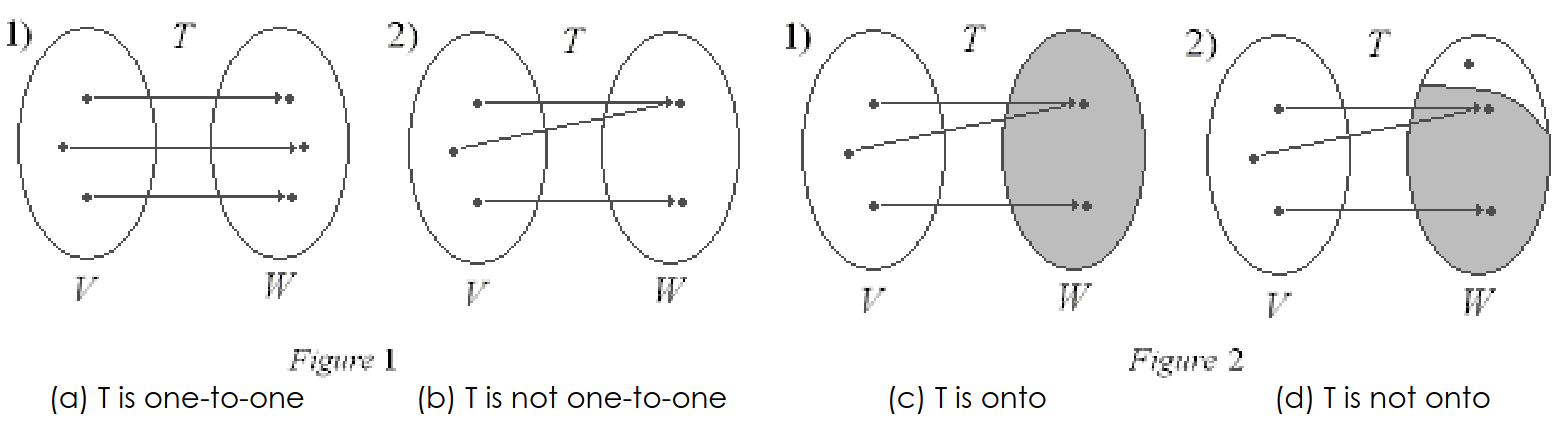
\includegraphics[width=1\linewidth]{linear-transformations.png}
\end{figure}

\begin{tikzpicture}
\node [rounded-box] (box){\begin{minipage}{0.975\textwidth}
    A linear transformation that is one-to-one and onto is called an \textbf{isomorphism} (iso = equal, morph = shape). If $V$ and $W$ are two vector spaces such that there is an isomorphism from $V$ to $W$, then $V$ is isomorphic to $W$:

    \vspace{-5pt}

    $$V \simeq W$$
\end{minipage}};
\node[rounded-box-title, left=10pt] at (box.north east) {Definition};
\end{tikzpicture}

\begin{tikzpicture}
\node [rounded-box] (box){\begin{minipage}{0.975\textwidth}
    Let $V, W$ be two finite-dimensional vector spaces (over the same field of scalars). Then $V$ is isomorphic to $W$ if and only if

    \vspace{-5pt}

    $$\text{dim}(V) = \text{dim}(W)$$
\end{minipage}};
\node[rounded-box-title, left=10pt] at (box.north east) {Theorem};
\end{tikzpicture}

\begin{tikzpicture}
\node [rounded-box] (box){\begin{minipage}{0.975\textwidth}
    Let $A$ be an $n \times n$ matrix. The following statements are equivalent:
    \begin{enumerate}
        \item $A$ is invertible.
        \item $A \mathbf{x} = \mathbf{b}$ has a unique solution for every $\mathbf{b} \in \mathbb{R}^n$.
        \item $A \mathbf{x} = \mathbf{0}$ has only the trivial solution.
        \item The reduced row echelon form of $A$ is $I_n$.
        \item $A$ is a product of elementary matrices.
        \item $\text{rank}(A) = n$.
        \item $\text{nullity}(A) = 0$.
        \item The column vectors of $A$ are linearly independent.
        \item The column vectors of $A$ span $\mathbb{R}^n$.
        \item The column vectors of $A$ form a basis for $\mathbb{R}^n$.
        \item The row vectors of $A$ are linearly independent.
        \item The row vectors of $A$ span $\mathbb{R}^n$.
        \item The row vectors of $A$ form a basis for $\mathbb{R}^n$.
        \item $\text{det}(A) \neq 0$.
        \item $0$ is not an eigenvalue of $A$.
        \item $T$ is invertible.
        \item $T$ is one-to-one.
        \item $T$ is onto.
        \item $\text{Ker}(T) = \{\mathbf{0}\}$.
        \item $\text{Range}(T) = W$.
    \end{enumerate}
\end{minipage}};
\node[rounded-box-title, left=10pt] at (box.north east) {The Fundamental Theorem of Invertible Matrices};
\end{tikzpicture}

\subsection{Inner Product Spaces}

\begin{tikzpicture}
\node [rounded-box] (box){\begin{minipage}{0.975\textwidth}
    The \textbf{inner product} takes pairs of vectors as inputs and produces scalars as outputs ($\mathbb{R}^n \times \mathbb{R}^n \rightarrow \mathbb{R}^n$):

    \vspace{-5pt}

    $$\mathbf{u}^T \mathbf{v} = \begin{bmatrix}
        u_1 & u_2 & u_3
    \end{bmatrix} \begin{bmatrix}
        v_1 \\ v_2 \\ v_3
    \end{bmatrix} = u_1 v_1 + u_2 v_2 + u_3 v_3$$
\end{minipage}};
\node[rounded-box-title, left=10pt] at (box.north east) {Definition};
\end{tikzpicture}

\begin{tikzpicture}
\node [rounded-box] (box){\begin{minipage}{0.975\textwidth}
    The \textbf{outer product} takes some vectors $\mathbf{u}, \mathbf{v}$ as inputs and produces matrices as outputs ($\mathbb{R}^n \times \mathbb{R}^n \rightarrow \mathbb{R}^{n \times n}$) such that every column is a multiple of the vector $\mathbf{u}$, and every row is a multiple of the vector $\mathbf{v}^T$:

    \vspace{-5pt}

    $$\mathbf{u} \mathbf{v}^T = \begin{bmatrix}
        u_1 \\ u_2 \\ u_3
    \end{bmatrix} \begin{bmatrix}
        v_1 & v_2 & v_3
    \end{bmatrix} = \begin{bmatrix}
        u_1 v_1 & u_1 v_2 & u_1 v_3 \\
        u_2 v_1 & u_2 v_2 & u_2 v_3 \\
        u_3 v_1 & u_3 v_2 & u_3 v_3
    \end{bmatrix}$$
\end{minipage}};
\node[rounded-box-title, left=10pt] at (box.north east) {Definition};
\end{tikzpicture}

\begin{tikzpicture}
\node [rounded-box] (box){\begin{minipage}{0.975\textwidth}
    An inner product on a vector space $V$ is an operation that assigns to every pair of vectors $\mathbf{u} , \mathbf{v} \in V$ a real number $\langle \mathbf{u}, \mathbf{v} \rangle$ such that the following properties hold for all vectors $\mathbf{u}, \mathbf{v}, \mathbf{w} \in V$ and all scalars $c$:

    \begin{itemize}
        \item $\langle \mathbf{u}, \mathbf{v} \rangle = \langle \mathbf{v}, \mathbf{u} \rangle$
        \item $\langle \mathbf{u}, \mathbf{v} + \mathbf{w} \rangle = \langle \mathbf{u}, \mathbf{v} \rangle + \langle \mathbf{u}, \mathbf{w} \rangle$
        \item $\langle c \mathbf{u}, \mathbf{v} \rangle = c \langle \mathbf{u}, \mathbf{v} \rangle$
        \item $\langle \mathbf{u}, \mathbf{u} \rangle \geq 0$
        \item $\langle \mathbf{u}, \mathbf{u} \rangle = 0$ if and only if $\mathbf{u} = \mathbf{0}$ \\
    \end{itemize}

    A vector space with such an inner product is called an \textbf{inner product space}.
\end{minipage}};
\node[rounded-box-title, left=10pt] at (box.north east) {Definition};
\end{tikzpicture}

\textbf{Example}: The dot product on $\mathbf{R}^n$ is an inner product.

\textbf{Example}: Continuous functions on an interval $[a, b]$ on the vector space $C[a, b]$ are inner products:

\begin{tikzpicture}
\node [rounded-box] (box){\begin{minipage}{0.975\textwidth}
    Let $f, g$ be continuous functions on an interval $[a, b]$. Then the inner product on the vector space $C[a, b]$ is defined as:

    $$
    \langle f, g \rangle = \int_a^b f(x) g(x) \, dx
    $$
\end{minipage}};
\node[rounded-box-title, left=10pt] at (box.north east) {Definition};
\end{tikzpicture}

\textbf{Example}: Let $f(x) = 1, g(x) = x^3$ on $C[0, 2]$. Their inner product is

$$
\langle f, g \rangle = \int_0^2 x^3 \, dx = \frac{1}{4} x^4 \Big{|}_0^2 = 4
$$

\begin{tikzpicture}
\node [rounded-box] (box){\begin{minipage}{0.975\textwidth}
    Let $\mathbf{u}, \mathbf{v}, \mathbf{w}$ be vectors in an inner product space $V$ and let $c$ be a scalar. Then

    \begin{itemize}
        \item $\langle \mathbf{u} + \mathbf{v}, \mathbf{w} \rangle = \langle \mathbf{u}, \mathbf{w} \rangle + \langle \mathbf{v}, \mathbf{w} \rangle$
        \item $\langle \mathbf{u}, c \mathbf{v} \rangle = c \langle \mathbf{u}, \mathbf{v} \rangle$
        \item $\langle \mathbf{u}, \mathbf{0} \rangle = \langle \mathbf{0}, \mathbf{v} \rangle = 0$
    \end{itemize}
\end{minipage}};
\node[rounded-box-title, left=10pt] at (box.north east) {Theorem};
\end{tikzpicture}

\begin{tikzpicture}
\node [rounded-box] (box){\begin{minipage}{0.975\textwidth}
    Let $\mathbf{u}, \mathbf{v}$ be vectors in an inner product space $V$. Then

    \begin{itemize}
        \item the \textbf{norm} or magnitude of $\mathbf{v}$ is: $|| \mathbf{v} || = \sqrt{\langle \mathbf{v}, \mathbf{v} \rangle}$
        \item their \textbf{distance} is: $d(\mathbf{u}, \mathbf{v}) = || \mathbf{u} - \mathbf{v} ||$
        \item $\langle \mathbf{u}, \mathbf{v} \rangle = 0 \iff \mathbf{u} \perp \mathbf{v}$
    \end{itemize}
\end{minipage}};
\node[rounded-box-title, left=10pt] at (box.north east) {Definition};
\end{tikzpicture}

Note: $|| \mathbf{v} ||$ is always defined, since $\langle \mathbf{v}, \mathbf{v} \rangle \geq 0$ by the definition of the inner product.

\textbf{Example}: Let $f(x) = 1, g(x) = x^3$ on $C[0, 2]$. Then their norms and distance are:

$$
|| f || = \sqrt{ \langle f, f \rangle } = \sqrt{ \int_0^2 f(x) f(x) \, dx } = \sqrt{ x \big{|}_0^2 } = \sqrt{2 - 0} = \sqrt{2}
\qquad
|| g || = \sqrt{ \langle g, g \rangle } = \sqrt{ \int_0^2 g(x) g(x) \, dx } = \sqrt{ x^7 / 7 \big{|}_0^2 } = \sqrt{2^7 / 7}
$$

$$
|| f - g || = \sqrt{ \langle f - g, f - g \rangle } = \sqrt{ \int_0^2 (f(x) - g(x))^2 \, dx }
$$

\textbf{Example}: Let $f(x) = 1, g(x) = \sin{x}$. In the vector space $C[0, \pi]$ with inner product $\langle f, g \rangle = \int_0^\pi f(x) g(x) \, dx$, are $f, g$ orthogonal?

\textbf{Example}: Let $f(x) = 1, g(x) = \sin{x}$. In the vector space $C[-\pi, \pi]$ with inner product $\langle f, g \rangle = \int_{-\pi}^\pi f(x) g(x) \, dx$, are $f, g$ orthogonal?

\begin{tikzpicture}
\node [rounded-box] (box){\begin{minipage}{0.975\textwidth}
    Let $\mathbf{u}, \mathbf{v}$ be vectors in an inner product space $V$. Then $\mathbf{u}, \mathbf{v}$ are orthogonal if and only if $|| \mathbf{u} + \mathbf{v} ||^2 = || \mathbf{u} ||^2 + || \mathbf{v} ||^2$.

    \begin{align}
        || \mathbf{u} + \mathbf{v} ||^2 & = \langle \mathbf{u} + \mathbf{v}, \mathbf{u} + \mathbf{v} \rangle \\
        & = \langle \mathbf{u} , \mathbf{u} \rangle + \langle \mathbf{u} , \mathbf{v} \rangle + \langle \mathbf{v} , \mathbf{u} \rangle + \langle \mathbf{v} , \mathbf{v} \rangle \\
        & = || \mathbf{u} ||^2 + 2 \langle \mathbf{u}, \mathbf{v} \rangle + || \mathbf{v} ||^2 \\
        & = || \mathbf{u} ||^2 + || \mathbf{v} ||^2 & \text{ if and only if } \langle \mathbf{u}, \mathbf{v} \rangle = 0
    \end{align}
\end{minipage}};
\node[rounded-box-title, left=10pt] at (box.north east) {The Pythagorean Theorem};
\end{tikzpicture}

\begin{paracol}{2}

\begin{tikzpicture}
\node [rounded-box] (box){\begin{minipage}{0.45\textwidth}
    Given a vector space $V$ with an inner product, a list $\{ v_1; v_2; \dots; v_n \}$ in $V$ is \textbf{orthogonal} if $\langle v_i, v_j \rangle = 0$ for all $i \neq j$. \\

    The list is orthonormal if it is orthogonal, and $|| v_i || = 1$ for all $i$.
\end{minipage}};
\node[rounded-box-title, left=10pt] at (box.north east) {Definition};
\end{tikzpicture}

\switchcolumn

\begin{tikzpicture}
\node [rounded-box] (box){\begin{minipage}{0.45\textwidth}
    Any orthogonal list of non-zero vectors is linearly independent.
\end{minipage}};
\node[rounded-box-title, left=10pt] at (box.north east) {Theorem};
\end{tikzpicture}

\end{paracol}
